\documentclass[letterpaper,12pt]{report}
\usepackage[top=1in, bottom=1in, left=1.5in, right=1.5in]{geometry}
\usepackage{fancyhdr,tocloft,natbib,url,graphicx,float,listings,sidecap,wrapfig}
\usepackage[font=small,labelfont=bf,labelsep=period]{caption}
\usepackage{tabularx, booktabs}
\usepackage{indentfirst}
\usepackage{setspace}
\usepackage{hyperref}
\usepackage[all]{hypcap}
\usepackage{qtree,algorithm,algorithmic}
\pagestyle{plain}
\fancyhf{}
\lhead{}
\chead{}
\rhead{}
\cfoot{\thepage}

%\floatstyle{boxed}
%\restylefloat{figure}

\hypersetup {
	colorlinks=false,
	pdfborder={0 0 0},
}

\setcounter{secnumdepth}{3}
\renewcommand*\thesection{\arabic{section}.}
\renewcommand*\thesubsection{\thesection \arabic{subsection}.}
\renewcommand*\thesubsubsection{\thesubsection \arabic{subsubsection}.}

\setcounter{tocdepth}{3}
\renewcommand\contentsname{}				% TOC title
\renewcommand\listfigurename{}			% LOF title
\renewcommand\listtablename{}				% LOT title
\setlength\cftaftertoctitleskip{-0.5in}
\setlength\cftafterloftitleskip{-0.5in}
\setlength\cftafterlottitleskip{-0.5in}

\renewcommand\bibsection{\section{References}}

\begin{document}

\hypersetup{pageanchor=false}
%%  COVER PAGE
\begin{titlepage}
	\begin{center}
		\vspace*{0.5in}
		\begin{doublespace}
			\LARGE \textbf{Metropolist} \\
			\vspace*{1in}
			\normalsize
			A Manuscript \\
			Submitted to \\
			the Department of Computer Science \\
			and the Faculty of the\\
			University of Wisconsin--La Crosse \\
			La Crosse, Wisconsin \\
			\vspace*{0.5in}
			by \\
			\large
			\textbf{Shizheng Yang} \\

			\vspace*{0.5in}
			\normalsize
			in Partial Fulfillment of the \\
			Requirements for the Degree of\\
			\Large{\textbf{Master of Software Engineering}} \\
			\normalsize
			May, 2019
		\end{doublespace}
	\end{center}
\end{titlepage}

\clearpage

%% SIGNATURE PAGE
\thispagestyle{empty}
\vspace*{0.3in}
\begin{center}
	\large{\textbf{Metropolist}} \\
	\vspace{0.75in}
	\normalsize{By Shizheng Yang}
\end{center}

\vspace{0.5in}
\noindent We recommend acceptance of this manuscript in partial fulfillment of this candidate's requirements for the degree of Master of Software Engineering in Computer Science. The candidate has completed the oral examination requirement of the capstone project for the degree. \\

\noindent
\begin{tabularx}{\textwidth}{p{3in}Xp{2in}}
	\rule{0pt}{50pt} & & \\
	\hrulefill & & \hrulefill \\
	Prof. Kasi Periyasamy & & Date \\
	Examination Committee Chairperson & & \\
	\rule{0pt}{50pt} & & \\
	\hrulefill & & \hrulefill \\
	Prof. Steven Senger & & Date \\
	Examination Committee Member & & \\
	\rule{0pt}{50pt} & & \\
	\hrulefill & & \hrulefill \\
	Prof. Kenny Hunt & & Date \\
	Examination Committee Member & & \\
\end{tabularx}

\clearpage

\hypersetup{pageanchor=true}
\setcounter{page}{1}
\pagenumbering{roman}
\renewcommand\arraystretch{1.5}

%% ABSTRACT
\section*{Abstract}
\addcontentsline{toc}{section}{Abstract}
Yang, Shizheng, ``Metropolist,'' Master of Software Engineering, May 2019, (Kenny Hunt, Ph.D.). \\

This manuscript describes the development of a web-based map generator, which allows the user to create randomly generated fantasy maps of cities and additionally allows the user to annotate and edit city elements at a fine granularity.
\clearpage

%%% ACKNOWLEDGEMENTS
\section*{Acknowledgements}
\addcontentsline{toc}{section}{Acknowledgments}
I would like to express my sincere appreciation to my project advisor Dr. Kenny Hunt for his invaluable guidance and untiring support. I would also like to express my thanks to the Department of Computer Science at the University of Wisconsin--La Crosse for providing the learning materials and computing environment for my project.
\clearpage

%% TABLE OF CONTENTS
\section*{Table of Contents}
\tableofcontents
\clearpage

%% LIST OF TABLES
\section*{List of Tables}
\addcontentsline{toc}{section}{List of Tables}
\listoftables
\clearpage

%% LIST OF FIGURES
\section*{List of Figures}
\addcontentsline{toc}{section}{List of Figures}
\listoffigures
\clearpage

%% GLOSSARY
\section*{Glossary}
\addcontentsline{toc}{section}{Glossary}
\subsubsection*{Ajax}
Ajax (short for asynchronous JavaScript and XML) is a set of web development techniques using many web technologies on the client side to create asynchronous web applications.

\subsubsection*{AngularJS}
AngularJS is a JavaScript-based open-source front-end web framework mainly maintained by Google and by a community of individuals and corporations to address many of the challenges encountered in developing single-page applications.

\subsubsection*{Application Programming Interface (API)}
In computer programming, an API is a set of subroutine definitions, communication protocols, and tools for building software. In general terms, it is a set of clearly defined methods of communication among various components.

\subsubsection*{Canvas}
Canvas is an HTML element which can be used to draw graphics via scripting (usually JavaScript). This can, for instance, be used to draw graphs, combine photos, or create simple (and not so simple) animations.

\subsubsection*{Endpoints}
Endpoints are important aspects of interacting with server-side web APIs, as they specify where resources lie that can be accessed by third-party software. Usually, the access is via a URI to which HTTP requests are posted, and from which the response is thus expected.

\subsubsection*{Express}
Express is a minimal and flexible Node.js web application framework that provides a robust set of features for web and mobile applications.

\subsubsection*{Functional Requirements}
In software engineering and systems engineering, a functional requirement defines a function of a system or its component, where a function is described as a specification of behavior between outputs and inputs.

\subsubsection*{Graphical User Interface (GUI)}
The GUI is a form of user interface that allows users to interact with electronic devices through graphical icons and visual indicators such as secondary notation, instead of text-based user interfaces, typed command labels or text navigation.

\subsubsection*{MongoDB}
MongoDB is a cross-platform document-oriented database program. Classified as a NoSQL database program, MongoDB uses JSON-like documents with schemata.

\subsubsection*{Node.js}
Node.js is an open-source, cross-platform JavaScript run-time environment that executes JavaScript code outside of a browser.

\subsubsection*{Non-Functional Requirements (NFR)}
In systems engineering and requirements engineering, a non-functional requirement is a requirement that specifies criteria that can be used to judge the operation of a system, rather than specific behaviors.

\subsubsection*{NoSQL}
NoSQL is an approach to database design that can accommodate a wide variety of data models, including key-value, document, columnar and graph formats.

\subsubsection*{Object Related Mapping (ORM)}
Object-relational mapping (ORM, O/RM, and O/R mapping tool) in computer science is a programming technique for converting data between incompatible type systems using object-oriented programming languages.

\subsubsection*{Representational State Transfer (REST)}
REST is a software architectural style that defines a set of constraints to be used for creating Web services.

\subsubsection*{Scalable Vector Graphics (SVG)}
SVG is an XML-based vector image format for two-dimensional graphics with support for interactivity and animation.

\subsubsection*{Single Page Application (SPA)}
A SPA is a web application or web site that interacts with the user by dynamically rewriting the current page rather than loading entire new pages from a server.

\subsubsection*{Software Life Cycle Model (SDLC)}
The SDLC is a term used in systems engineering, information systems, and software engineering to describe a process for planning, creating, testing, and deploying an information system.

\subsubsection*{Stakeholder}
The stakeholder (also project stakeholder) is an individual, group, or organization, who may affect, be affected by, or perceive itself to be affected by a decision, activity, or outcome of a project.

\subsubsection*{Web API}
A Web API is an application programming interface for either a web server or a web browser.

\clearpage

\setcounter{page}{1}
\pagenumbering{arabic}

\IfFileExists{section01/section}{\section{Introduction}
\label{sec:Introduction}

\subsection{Background}
Generating content for computer games, CGI effects, feature films, print media, or Role-playing games is a significant bottleneck in terms of effort and resources. A typical game contains many thousands of audio files, images, textures, and 3D models. Procedurally generated content provides a cost-effective alternative to the manual creation of models, textures, images, and sound assets and can expand playability beyond what is otherwise possible. The video game ``No Man's Sky,'' for example, was released in 2016 and relied on procedural asset generation to create over 18 quintillion planets each of which has a unique ecosystem composed of flora and fauna. Such a scale is, of course, beyond the reach of any manually created system. Figure \ref{Screenshot NoManSky} is a screenshot of a planetary terrain region of ``No Man's Sky.''

\begin{figure}[!htb]
\centering
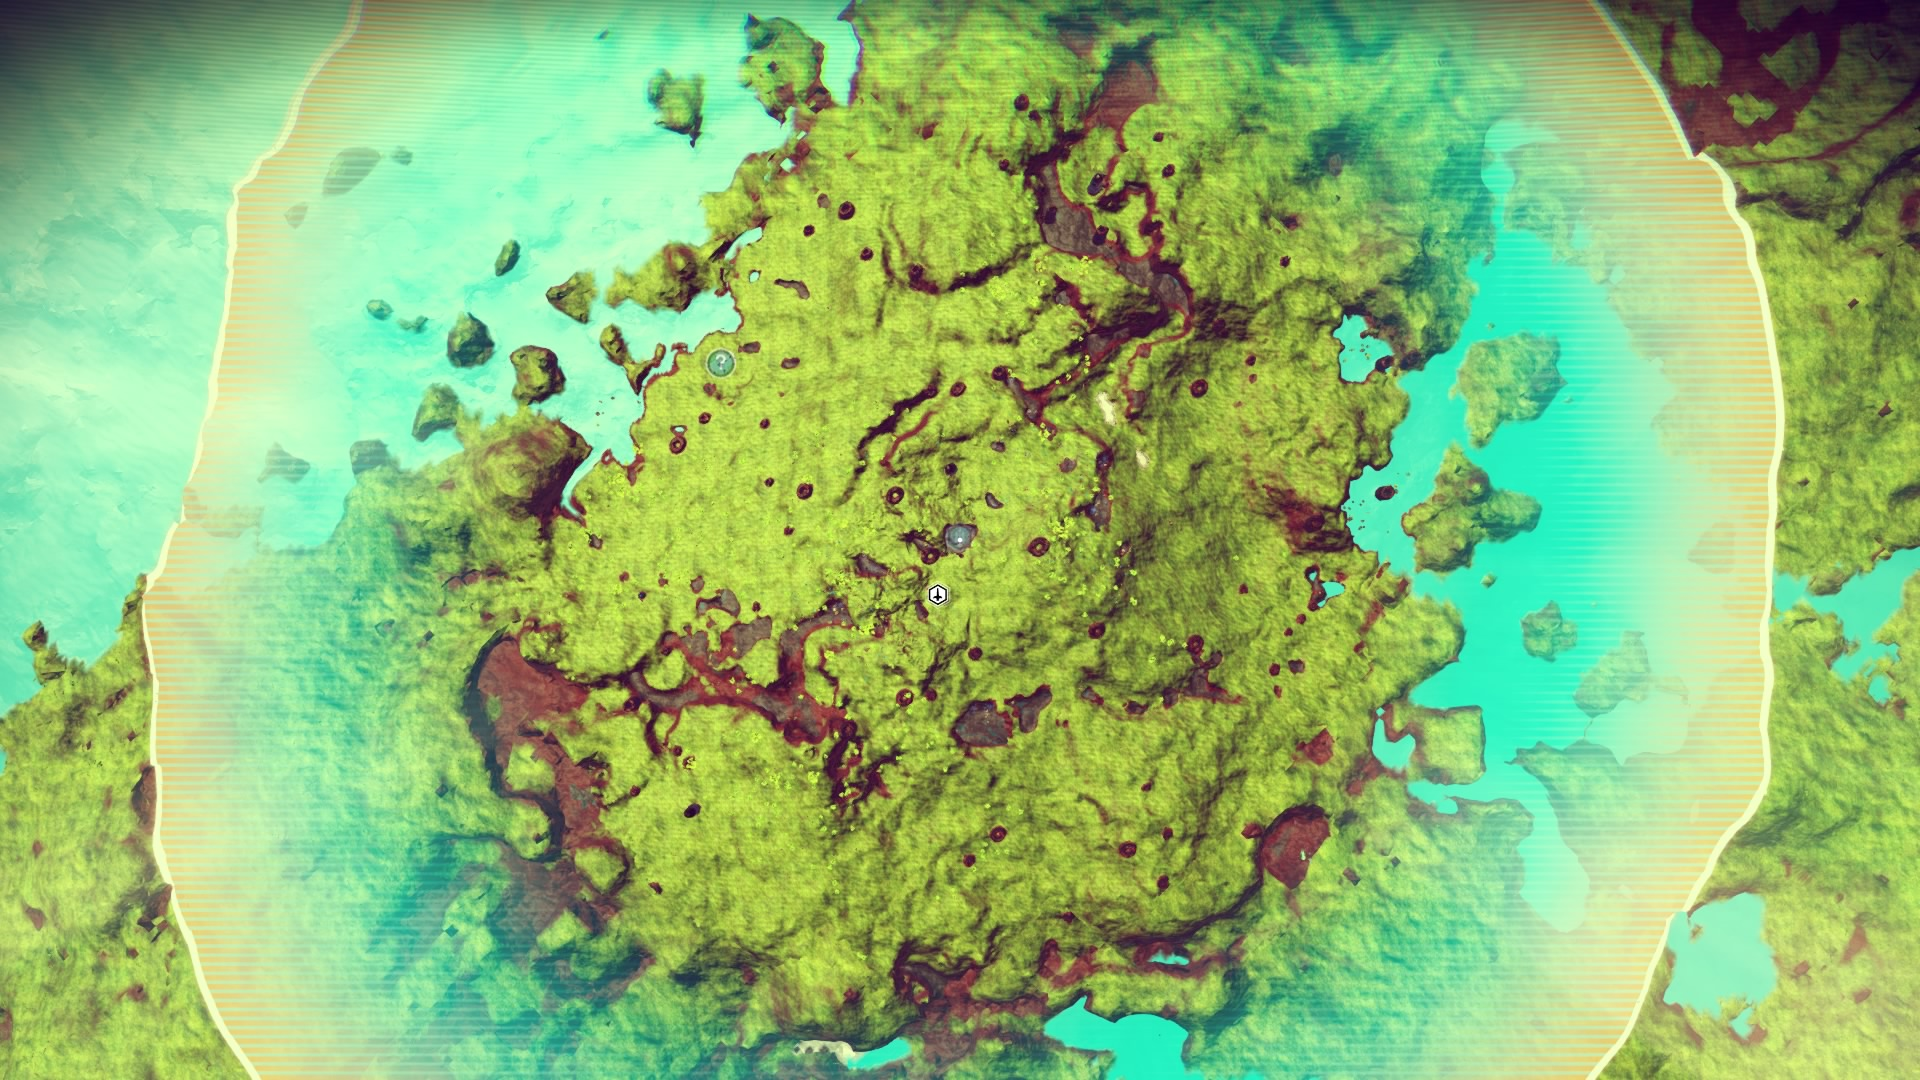
\includegraphics[width=\textwidth]{section01/assets/screenshot_NoManSky.jpg}
\caption[A screenshot of a planetary terrain region of ``No Man's Sky'']{\label{Screenshot NoManSky}A screenshot of a planetary terrain region of ``No Man's Sky''}
\end{figure}

\subsection{Similar Systems}
% The goal of this project is to automatically generate city maps for use in Role-playing games or world building narratives.
\subsubsection{Minecraft}
``Minecraft'' is a computer game that can produce massive worlds composed of fine details, like elaborate cliff faces and waterfalls. Moreover, it relies on procedural generation, which automatically creates environments and objects that are at once random but guided by rules that maintain a consistent logic. Mountains are always rocky and sprinkled with snow, for example, while the low lands are typically full of grass and trees. Figure \ref{Screenshot Minecraft} is a screenshot of ``Minecraft.''

\begin{figure}[!htb]
\centering
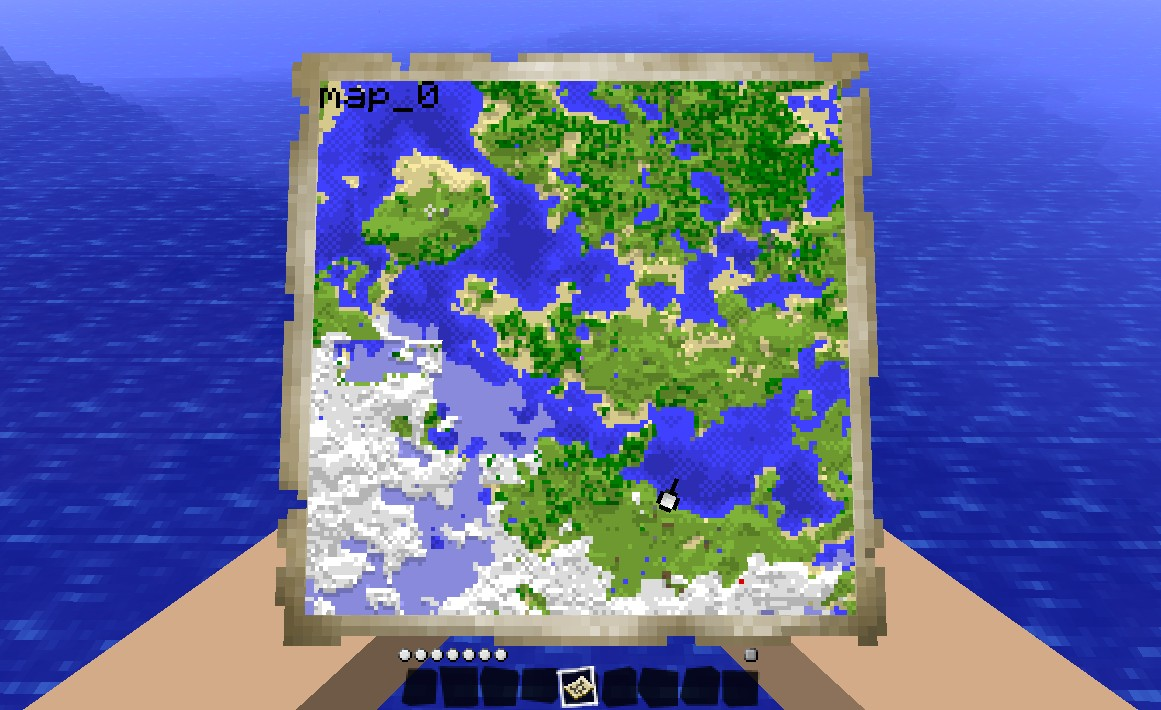
\includegraphics[width=\textwidth]{section01/assets/screenshot_Minecraft.jpg}
\caption[A screenshot of ``Minecraft'']{\label{Screenshot Minecraft}A screenshot of ``Minecraft''}
\end{figure}

\subsubsection{Medieval Fantasy City Generator(MFCG)}
The ``Medieval Fantasy City Generator(MFCG)'' is a web application. This application generates a random medieval city layout of a requested size: small, medium or large, which is made up of different types of regions, and the generation method is stochastic. Furthermore, elements are provided for the user to add to the city, such as farm fields, citadel, plaza, temple, river, coast and so on. Because of the premise of medieval fantasy, the map always includes the walls and castle, but the user can decide whether to display them. It allows the user to edit the map to modify unsatisfying layers using a warping tool. The author also mentioned that the goal of the application is to produce a nice looking map, not an accurate model of a city. Finally, the user can save the map as an image in the ``png'' or ``svg'' format by using the export feature. Figure \ref{Screenshot MFCG} is a screenshot of MFCG.

\begin{figure}[!htb]
\centering
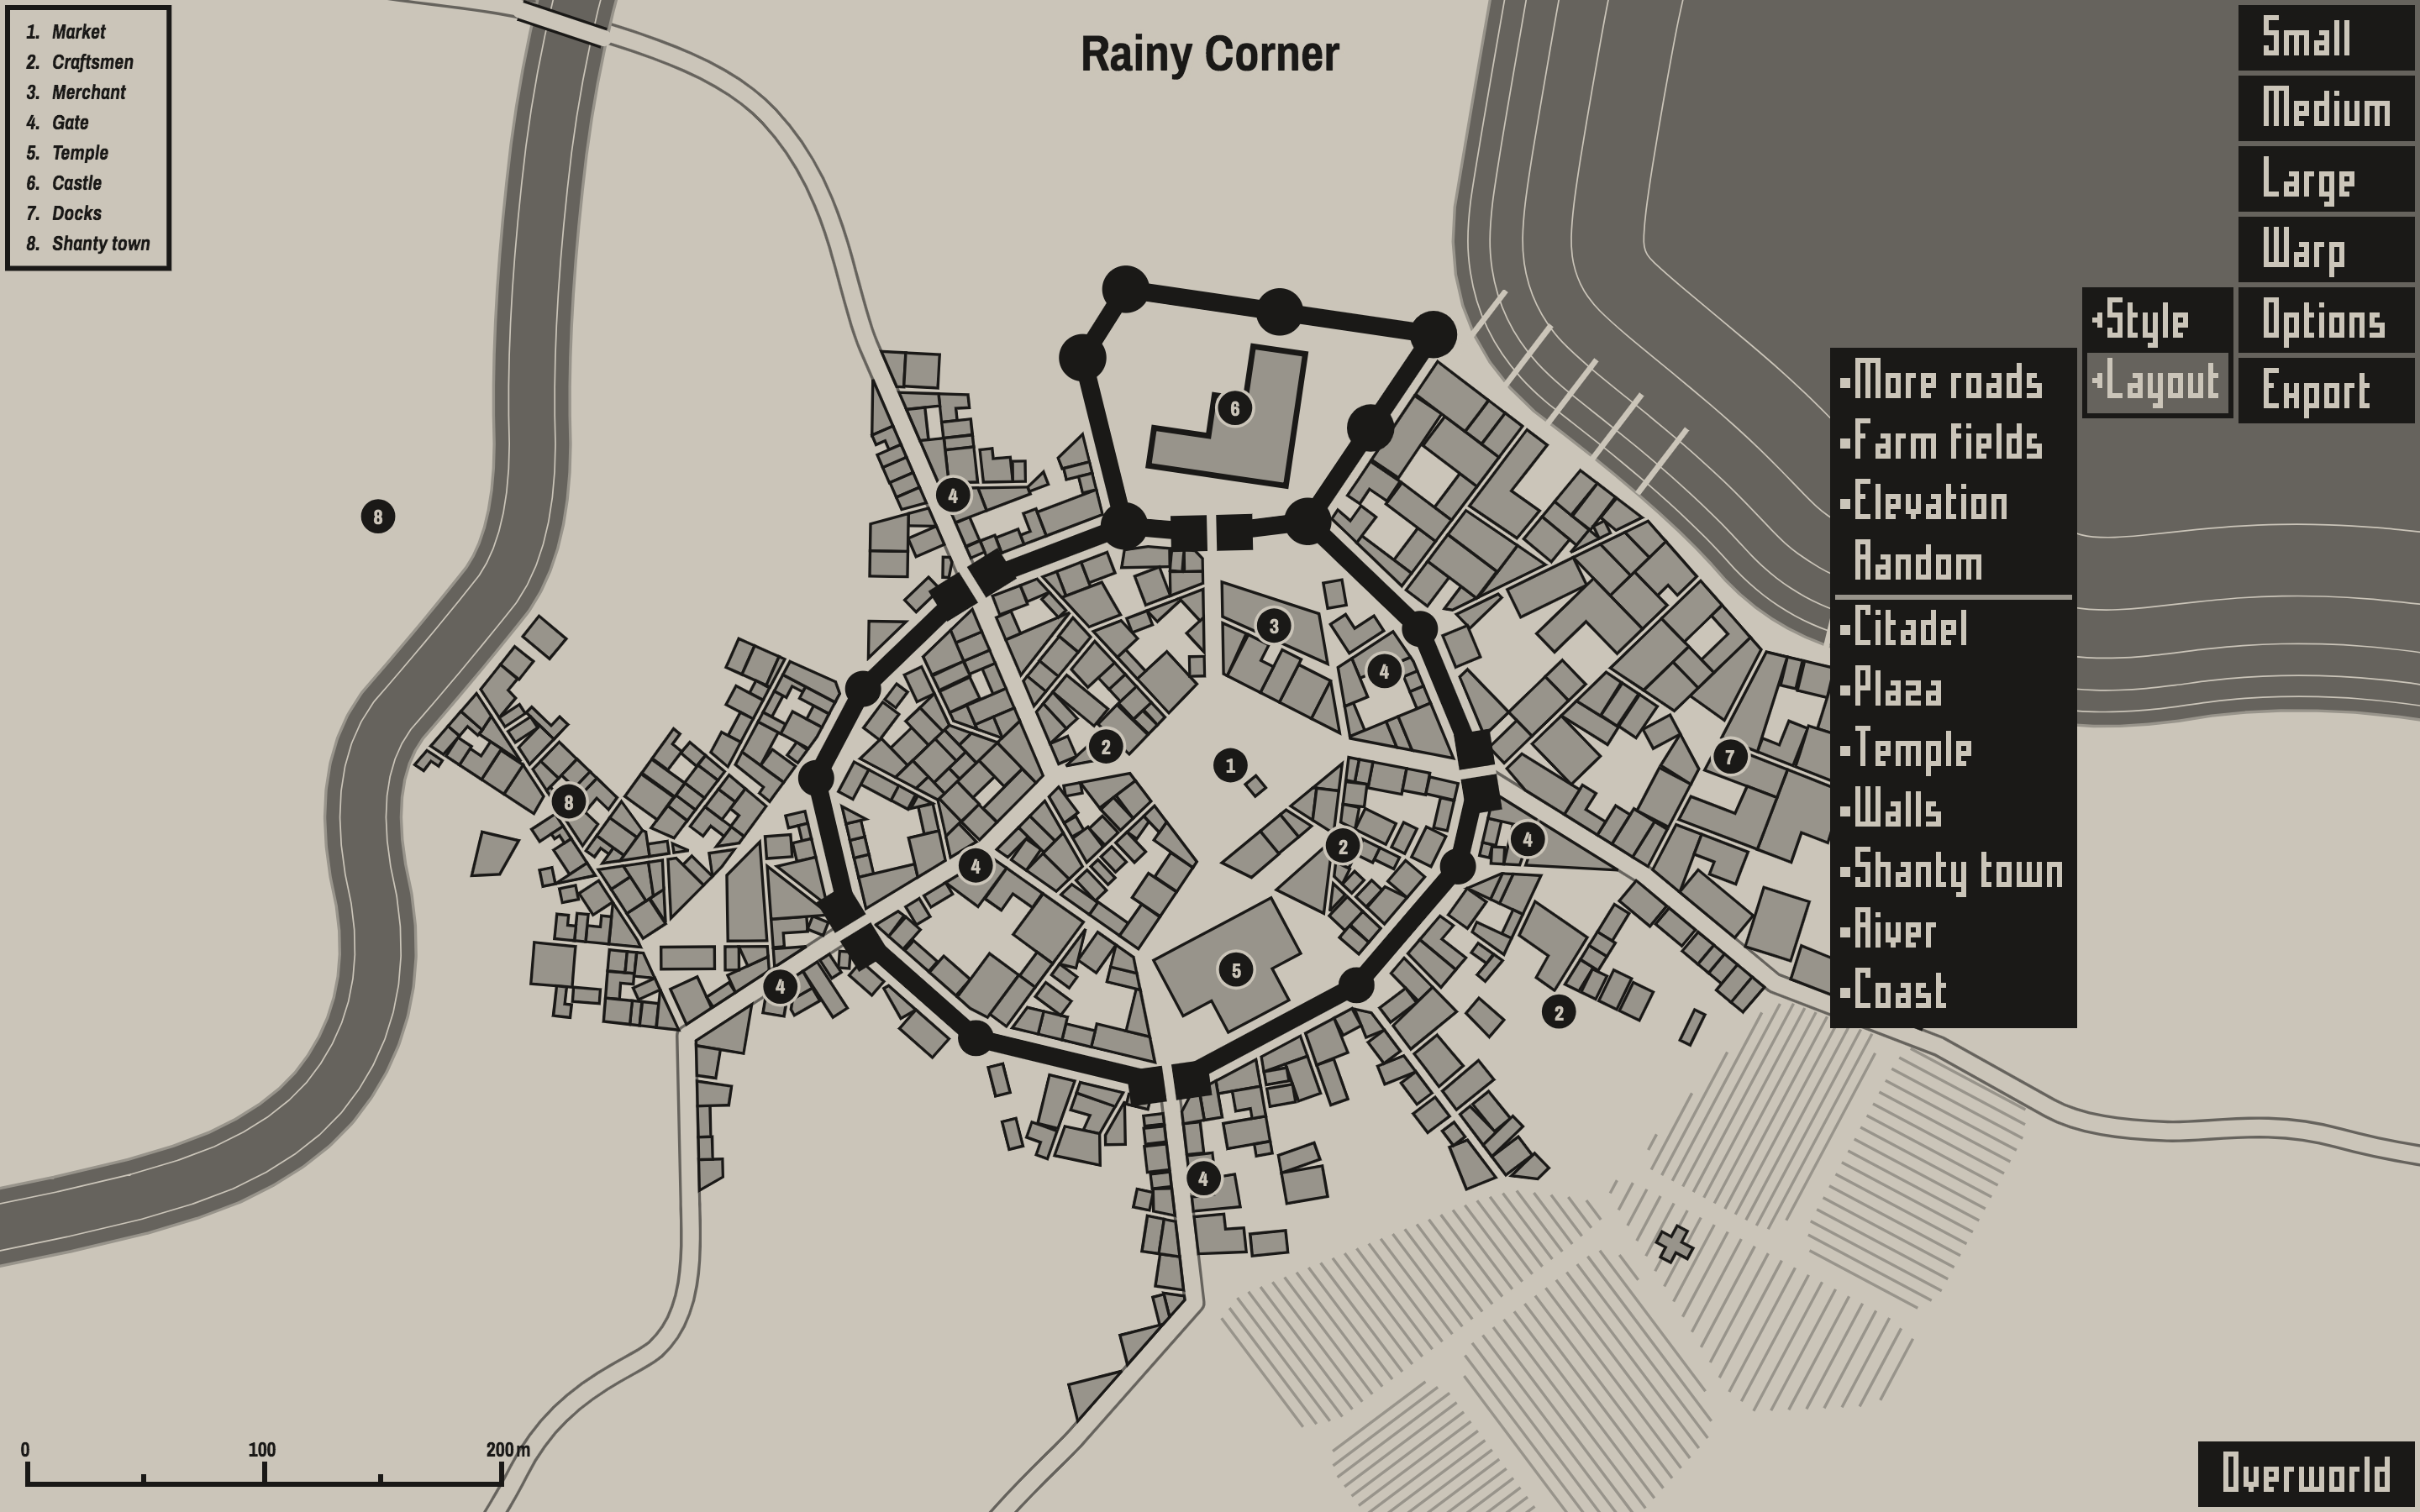
\includegraphics[width=\textwidth]{section01/assets/screenshot_MFCG.png}
\caption[A screenshot of the Medieval Fantasy City Generator]{\label{Screenshot MFCG}A screenshot of the Medieval Fantasy City Generator}
\end{figure}

\subsubsection{Azgaar's Fantasy Map Generator(FMG)}
The ``Azgaar's Fantasy Map Generator(FMG)'' is another similar system, which is a larger scale world map. The size of the map made by FMG is not just an island, but a random fantasy map represents a pseudo-medieval world. Just like the real world, the map generated by FMG has constraints that the continent is always surrounded by the ocean and will never touch the border of the map. Although it is a randomly generated map, it is still based on real-world rules. While its most prominent feature is that the user can choose the type of map he likes, which provides the following 5 map types: political, cultural, height, biomes and pure landmass. It also supports user-defined map type, and the user can add additional layers on existing map layers: rivers, temperature, and population. Also, it allows the user to annotate and edit the map using various such editors: layout, style, template, scale, countries, or cultural. It also supports exporting the map in the ``png'' or ``svg'' format, but unlike the previous application, if the user wants to come back to edit the map in the future, he can save it in the ``map'' format. Figure \ref{Screenshot FMG} is a screenshot of FMG.

\begin{figure}[!htb]
\centering
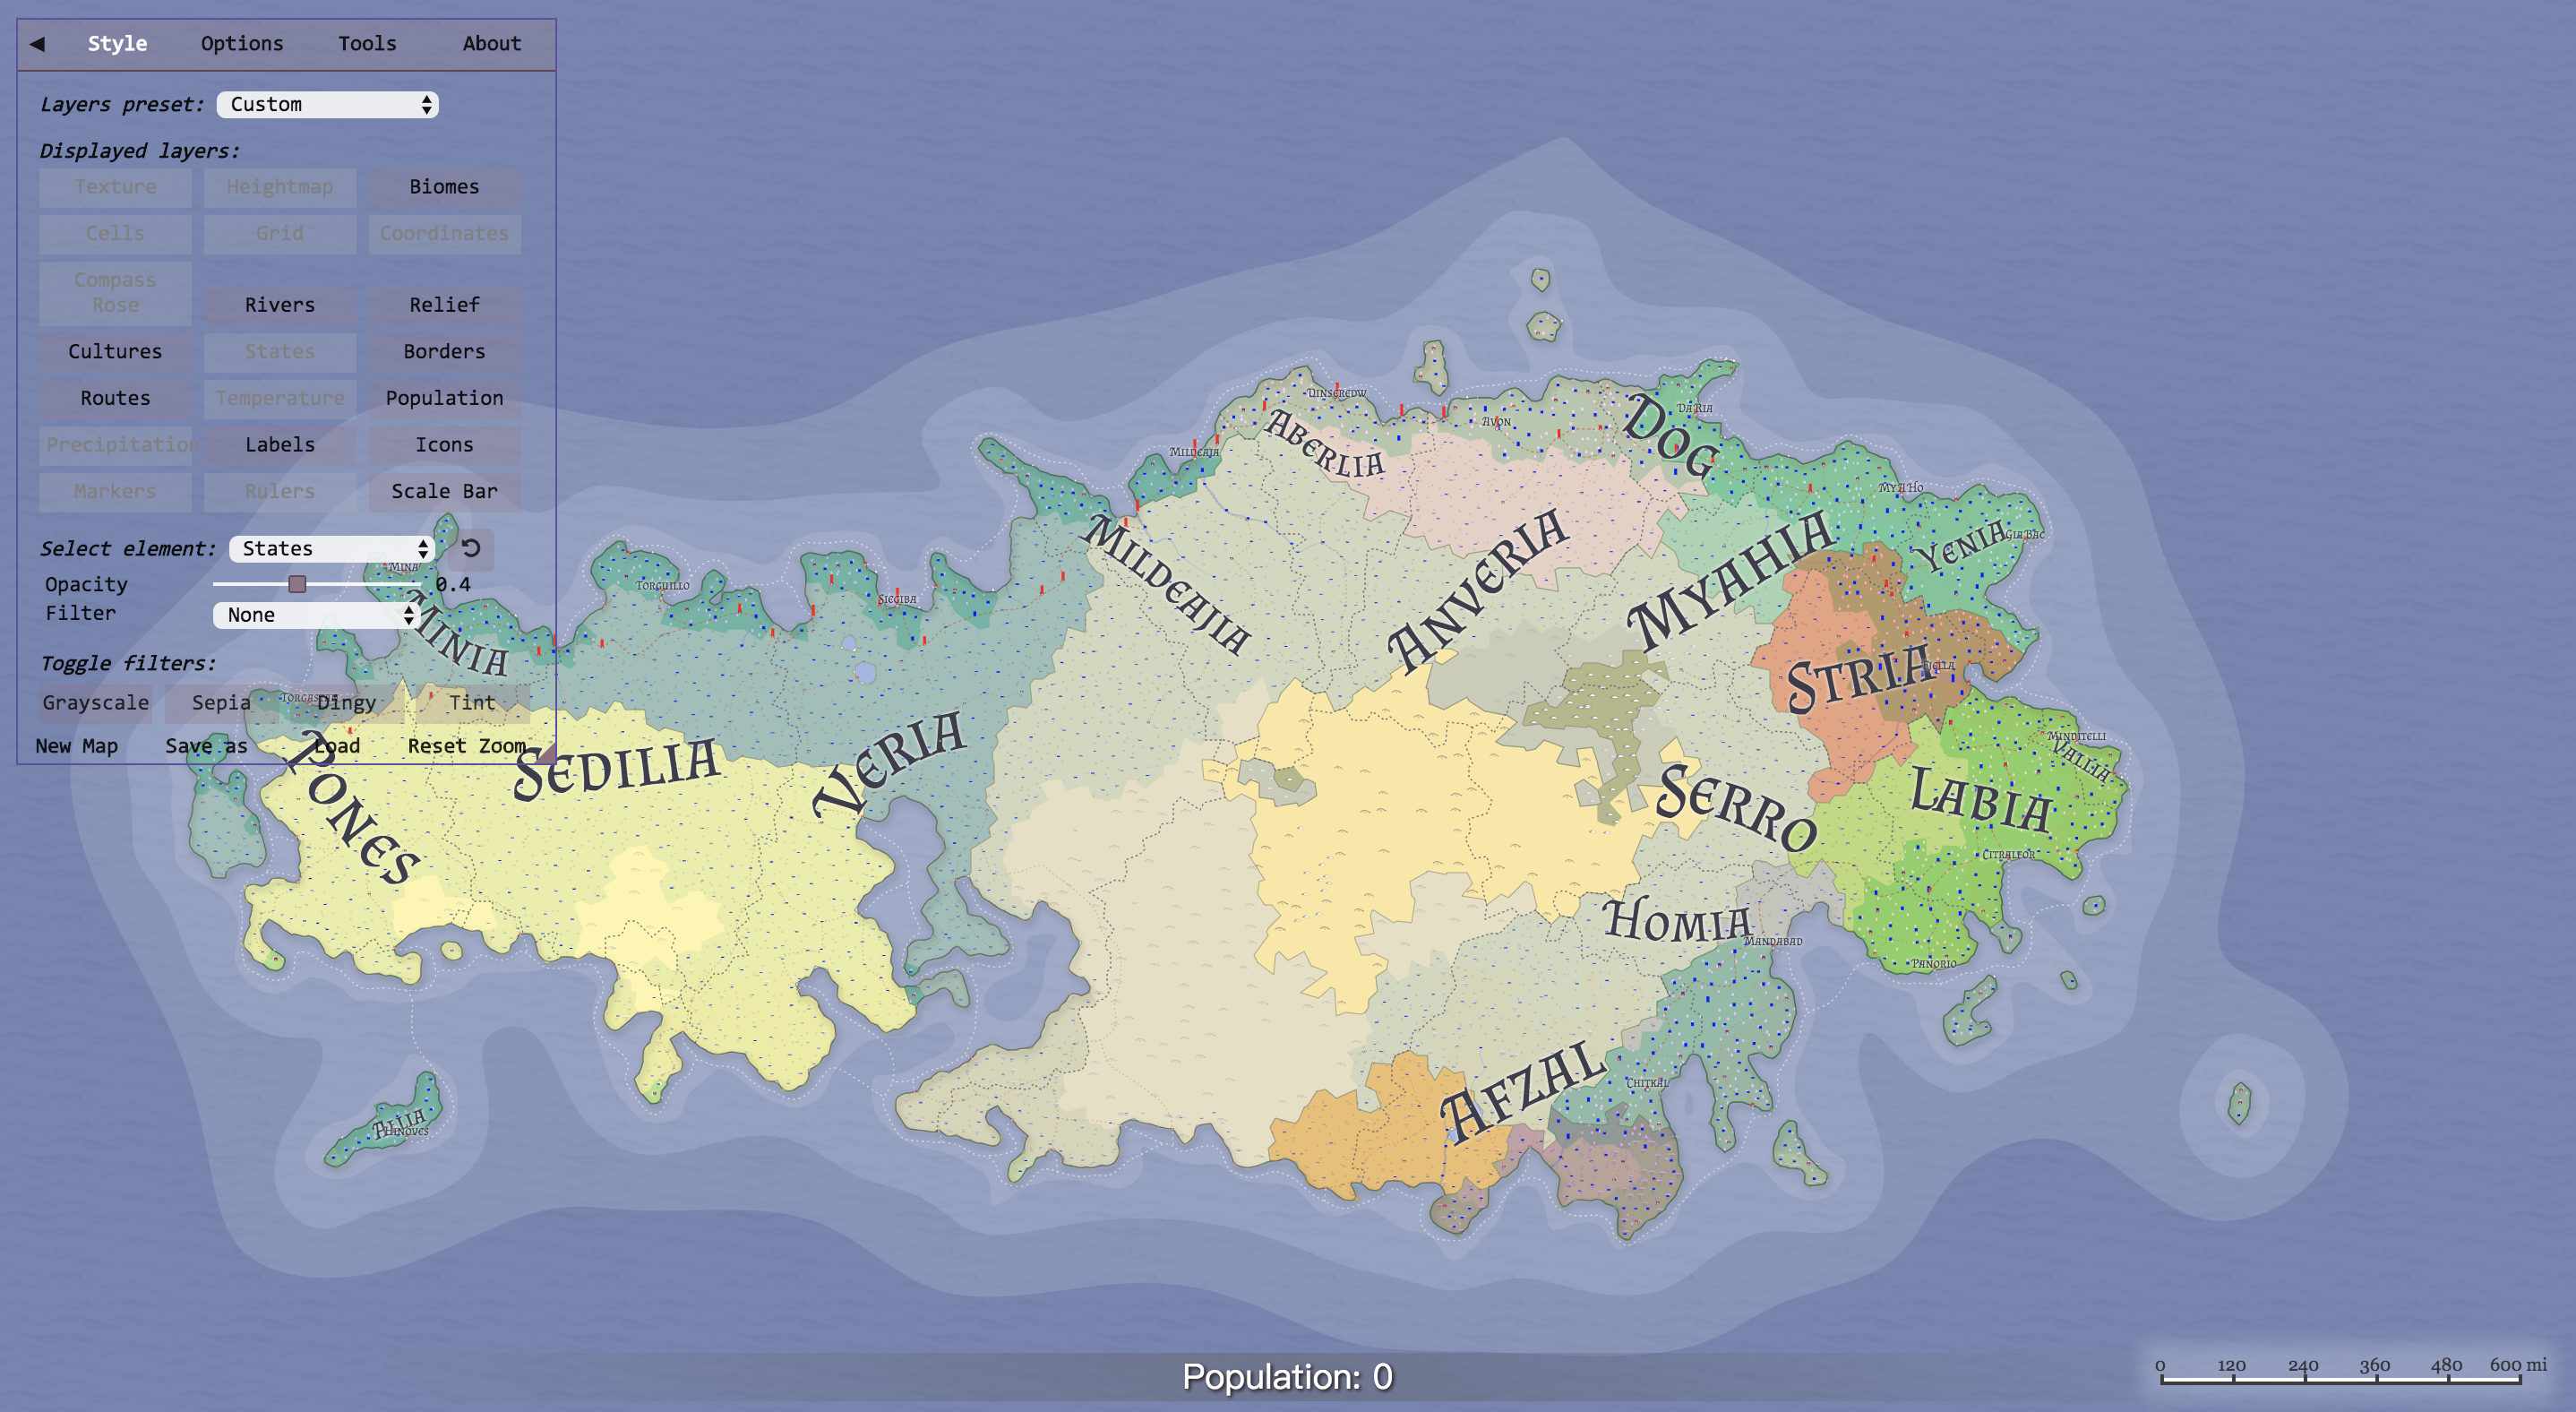
\includegraphics[width=\textwidth]{section01/assets/screenshot_FMG.png}
\caption[A screenshot of the Azgaar's Fantasy Map Generator]{\label{Screenshot FMG}A screenshot of the Azgaar's Fantasy Map Generator}
\end{figure}

\subsection{Project Goal}
The goal of this project is to automatically generate city maps for use in Role-playing games (RPG) or Worldbuilding narratives. While the ultimate goal of this project is to procedurally replicate maps of a quality similar to the best cartographic hand-created maps by expert artists, we have obtained a modest approximation to the desired level of quality. Our system will have the essential features, such as: allowing the user to annotate or edit, allowing the user to export the map as an image in the ``png'' or ``svg'' format, allowing the user to save it to a database and retrieve it. Figure \ref{Screenshot Metropolist} is a screenshot of our current project.

\begin{figure}[!htb]
\centering
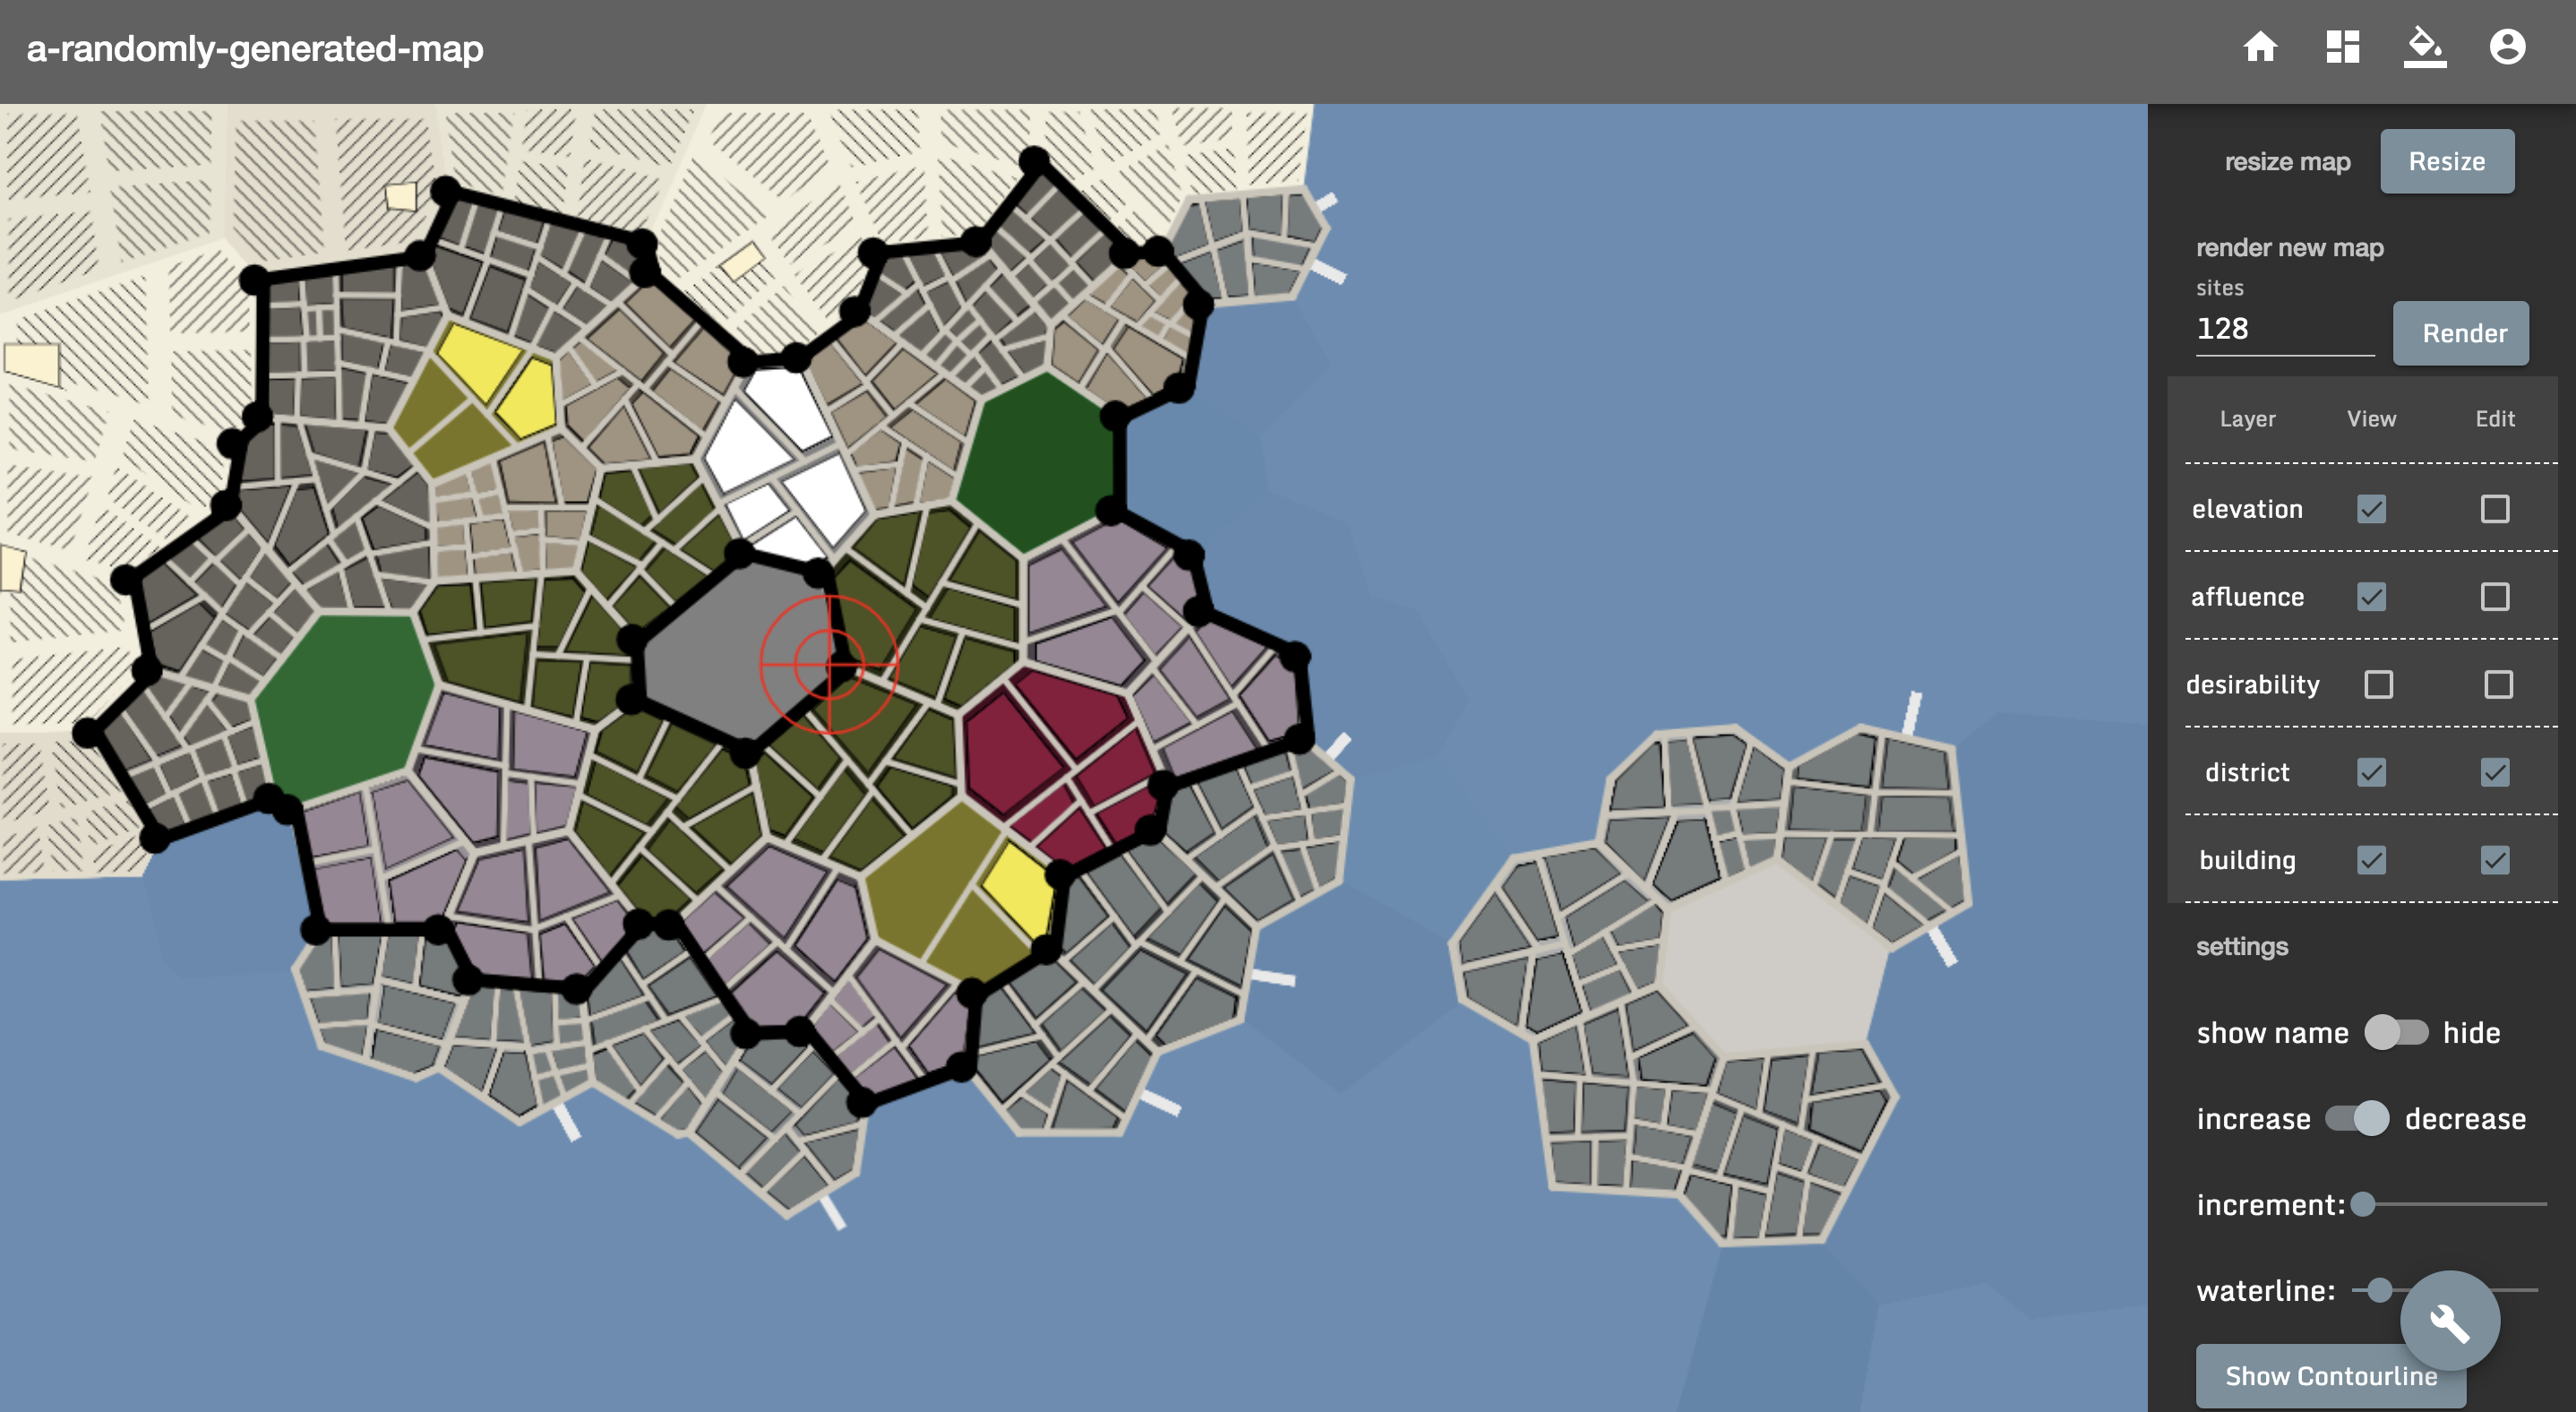
\includegraphics[width=\textwidth]{section01/assets/screenshot_Metropolist.png}
\caption[A screenshot of the current project]{\label{Screenshot Metropolist}A screenshot of the current project}
\end{figure}
}{}\clearpage
\IfFileExists{section02/section}{\section{Requirements}
\label{sec:Requirements}

\subsection{Overview} 
This gives a brief overview of this section.

\subsection{Point 1}
This subsection gives a great deal of precise description supporting point 1.  For example,
Figure \ref{State Chart 2} explains in great detail a state chart.

\begin{figure}[htb]
\centering
\includegraphics[width=.5\textwidth]{section02/assets/sample_image.png}
\caption[Short Caption 2]{\label{State Chart 2}State Chart Diagram}
\end{figure}

\subsection{Point 2}
This gives Point 2
}{}\clearpage
\IfFileExists{section03/section}{\section{Design}
\label{sec:Design}

\subsection{Architecture Design}
Because we selected the web application model from the beginning, so the classic client-server architecture was quickly adopted, which is a distributed application structure that partitions tasks or workloads between the providers of a resource or service, called servers, and service requesters, called clients. In theory, any device connected to the Internet can try to access and obtain the resources or services of the server while the server is running normally. Figure \ref{Client-Server Architecture} shows how it works.

\begin{figure}[htb]
\centering
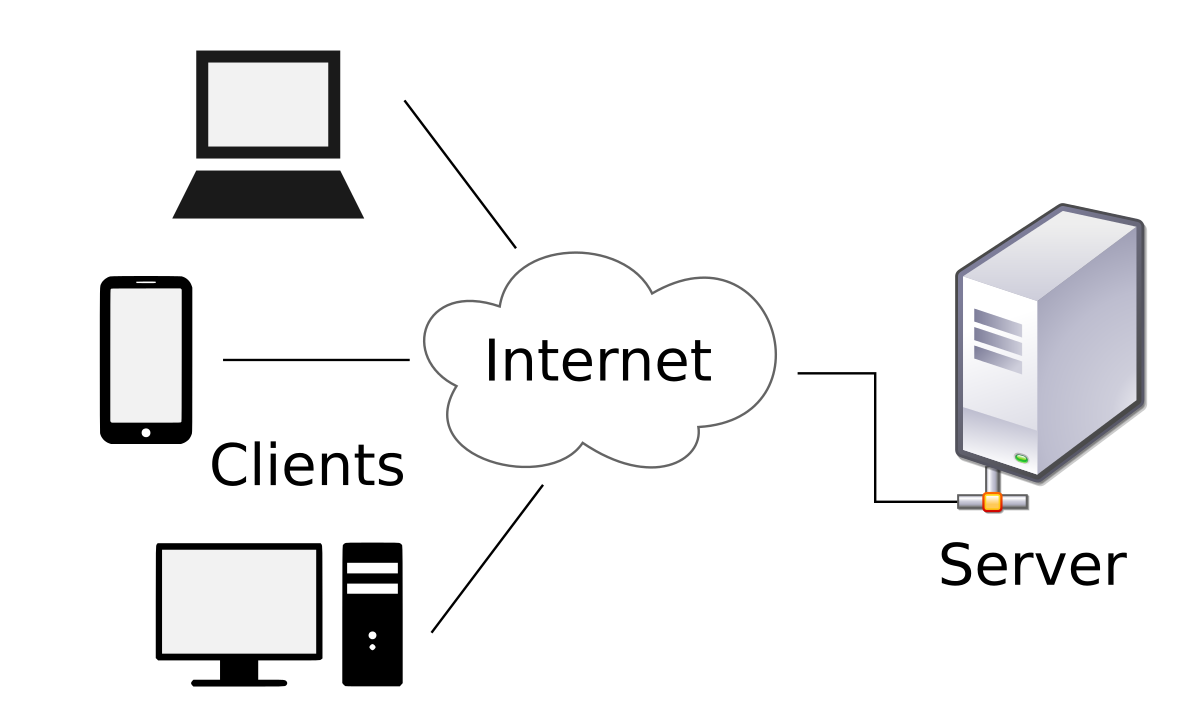
\includegraphics[width=\textwidth]{section03/assets/client_server.png}
\caption[the Architecture of Client-Server Model]{\label{Client-Server Architecture}the Architecture of Client-Server Model}
\end{figure}

Based on the client-server structure, we have detailed its component structures below:
\subsubsection{Web Browser or Client}
The web browser or client is the interface rendition of a web app functionality, with which the user interacts with. This content delivered to the client can be developed using HTML, JavaScript, and CSS and doesn’t require operating system related adaptations. In essence, the web browser or client manages how end users interact with the application.

There are three, well-known Web Application Architecture types available in the modern tech landscape: Single Page Applications (SPA), Microservices, and Serverless Architectures. Considered the needs of the project and the choice of the Software Development Life Cycle (SDLC) model, we chose the SPA architecture.

The SPA model interacts with the user in a more dynamic fashion by providing updated content within the current page, rather than loading entirely new pages from the server with each action from the user. It helps prevent interruptions in the user experience, transforming the behavior of the application such that it resembles a traditional desktop application.

\subsubsection{Web Application Server}
The web application server manages business logic and data persistence and can be built using PHP, Python, Java, Ruby, .NET, Node.js, among other languages. It’s comprised of at least a centralized hub or control center to support multi-layer applications. The essential purpose of a web server architecture is to complete requests made by clients for a website. The clients are typically browsers and mobile apps that make requests using secure HTTPs protocol, either for page resources or a REST API.

Since the focus of this project is on the client side (frontend), which is the map generator (written in JavaScript), so we chose the Node.js Express framework. Moreover, the Node.js is written using JavaScript and is the same technology as frontend components, which makes it easier for the developer to program backend services and frontend user interfaces. It also provides consistency, code sharing and reusability, simple knowledge-transfer, and a large number of free tools. These benefits bring flexibility and efficiency when building this project.

\subsubsection{Database Server}
The database server provides and stores relevant data for the application. Additionally, it may also supply the business logic and other information that is managed by the web application server. There are multiple popular database systems available: Oracle, MySQL, Microsoft SQL Server, PostgreSQL, MongoDB, MariaDB, DB2, and SAP HANA.

Because of the project involves a small number of entities and the relationships among entities are not complicated, and the choice of the Software Development Life Cycle (SDLC) model, we chose the MongoDB, which is dynamic, flexible and easy to get started. It also provides high performance, high availability, and high scalability. What's more, our main purpose is to save maps and implement basic CRUD (create, retrieve, update, delete) operations of the database. As MongoDB is a schema-less database (written in C++), we can serialize the map data to JSON, send it to MongoDB and then save it.

\subsection{Database Design}
NoSQL, which stands for "not only SQL," is an approach to database design that can accommodate a wide variety of data models, including key-value, document, columnar and graph formats. MongoDB is a type of NoSQL database. A record in MongoDB is a document, which is a data structure composed of field and value pairs. MongoDB documents are similar to JSON objects, the values of fields may include other documents, arrays, and arrays of documents.

Firstly, we thought there should be two entities: the user and the map. A user can have many maps, but a map can only belong to one user. Thus, the relationship between the user and the map should be One-to-Many.

MongoDB provides two ways of data modeling: Embedded Data Modeling and Normalized Data Modeling. Using Embedded Data Modeling, we may embed related data in a single structure or document, which means we should store maps in the user schema. But the data of the map is relatively large, in general, the CRUD operations will be slower, and the map cannot exist as a separate entity, so this one is beyond our consideration.

Normalized Data Modeling provides One-to-One relationship and One-to-Many relationship,
here we chose the Normalized One-to-Many structure.

Figure \ref{ER Diagram} shows the relationship between the ``user'' and the ``map''.

\begin{figure}[htb]
\centering
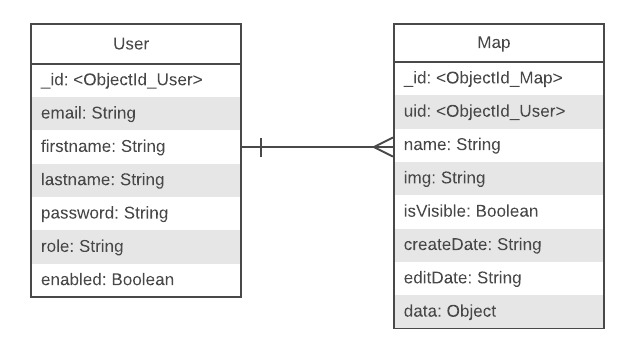
\includegraphics[width=\textwidth]{section03/assets/ER_Diagram.png}
\caption[ER Diagram]{\label{ER Diagram}ER Diagram}
\end{figure}

\subsection{REST API Design}
REST is the acronym for Representational State Transfer. It is an architectural style for distributed hypermedia systems and was first presented by Roy Fielding in 2000 in his famous dissertation.
%[https://www.ics.uci.edu/~fielding/pubs/dissertation/rest_arch_style.htm]

Like any other architectural style, REST also does have it’s own 6 guiding constraints which must be satisfied if an interface needs to be referred as RESTful. These principles are listed below:
\begin{enumerate}
  \item Client–server - By separating the user interface concerns from the data storage concerns, we improve the portability of the user interface across multiple platforms and improve scalability by simplifying the server components
  \item Stateless - Each request from a client to server must contain all of the information necessary to understand the request, and cannot take advantage of any stored context on the server. Session state is therefore kept entirely on the client
  \item Cacheable – Cache constraints require that the data within a response to a request be implicitly or explicitly labeled as cacheable or non-cacheable. If a response is cacheable, then a client cache is given the right to reuse that response data for later, equivalent requests
  \item Uniform interface – By applying the software engineering principle of generality to the component interface, the overall system architecture is simplified and the visibility of interactions is improved.
  \item Layered system – The layered system style allows an architecture to be composed of hierarchical layers by constraining component behavior such that each component cannot ``see'' beyond the immediate layer with which they are interacting
  \item Code on demand (optional) – REST allows client functionality to be extended by downloading and executing code in the form of applets or scripts. This simplifies clients by reducing the number of features required to be pre-implemented
\end{enumerate}

Based on these principles, we have designed the APIs shown in Table \ref{REST API Design Table}.
\begin{table}[htb]
  \centering
  \begin{tabularx}{\textwidth}{>{\raggedright}cXX} % way of defining a fix columns width
    \toprule[1.5pt]
    \textbf{HTTP Verb} & \textbf{URI} & \textbf{Description}
    \\ \midrule[1.5pt]
    % POST & /metro/auth/signup & Sign up for a new account
    % \\ \midrule
    % POST & /metro/auth/login & Log in to the system
    % \\ \midrule
    % POST & /metro/auth/logout & Log out of the system
    % \\ \midrule
    GET & /metro/api/v1/users & Get a list of all users
    \\ \midrule
    GET & /metro/api/v1/users/\{id\} & Get the user with \{id\}
    \\ \midrule
    GET & /metro/api/v1/users/\{uid\}/ maps & Get a list of all maps of the user with \{uid\}
    \\ \midrule
    PATCH & /metro/api/v1/users/\{id\}/ password & Verify the password of the user with \{id\}
    \\ \midrule
    PUT & /metro/api/v1/users/\{id\}/ password & Update the password of the user with \{id\}
    \\ \midrule
    PUT & /metro/api/v1/users/\{id\}/ email & Update the email of the user with \{id\} \\ \midrule
    PUT & /metro/api/v1/users/\{id\}/ name & Update the name of the user with \{id\} \\ \midrule
    PUT & /metro/api/v1/users/\{id\}/ enabled & Update the enabled of the user with \{id\}
    \\ \midrule
    GET & /metro/api/v1/maps/\{id\} & Get the map with \{id\}
    \\ \midrule
    GET & /metro/api/v1/maps/ ?page=\{page\}\&limit=\{limit\} & Get a list of \{limit\} maps on page \{page\}
    \\ \midrule
    POST & /metro/api/v1/maps & Add a new map to the database
    \\ \midrule
    PUT & /metro/api/v1/maps/\{id\} & Update the map with \{id\}
    \\ \midrule
    DELETE & /metro/api/v1/maps/\{id\} & Delete the map with \{id\}
    \\ \bottomrule[1.5pt]
  \end{tabularx}
  \caption[REST API Design Table]{REST API Design Table}
  \label{REST API Design Table}
\end{table}

\subsection{Map Generator Design}
}{}\clearpage
\IfFileExists{section04/section}{\section*{Section01}																	
\label{sec:Section01}
\addcontentsline{toc}{section}{Section01}

\subsection{Overview} 
This gives a brief overview of this section.

\subsection{Point 1}
This subsection gives a great deal of precise description supporting point 1.  For example,
Figure \ref{State Chart} explains in great detail a \index{state chart}state chart.

\begin{figure}[htb]
\centering
\includegraphics[width=.5\textwidth]{section01/assets/sample_image.png}
\caption[Short Caption]{\label{State Chart}State Chart Diagram}
\end{figure}

\subsection{Point 2}
This gives Point 2
}{}\clearpage

%% BIBLIOGRAPHY
\bibliography{capstone}
\bibliographystyle{plain}
\label{sec:bibliougraphy}
\clearpage

%%% APPENDICES
\section{Appendices}
\label{sec:appendices}
\clearpage

\end{document}
